\documentclass[a4paper,fleqn,10pt]{article}
\usepackage{graphicx}
\usepackage[utf8]{inputenc}

\renewcommand{\labelenumii}{\theenumii}
\renewcommand{\theenumii}{\theenumi.\arabic{enumii}.}

%%%%%%%%%%%%%%%%%%%%


\usepackage[]{geometry}
\usepackage[latin1]{inputenc}
\usepackage[UKenglish]{babel}
\usepackage[UKenglish]{isodate}
\usepackage{amsmath}
\usepackage{amsfonts}
\usepackage{amssymb}
\usepackage{amsthm}
\usepackage{graphicx}
\usepackage{chngpage}
\usepackage{calc}
\PassOptionsToPackage{hyphens}{url}
\usepackage{hyperref}
\usepackage[nameinlink]{cleveref}
\usepackage{fancyhdr}
\usepackage{titletoc}
\usepackage[explicit]{titlesec}
\usepackage{natbib}
\usepackage[dvipsnames]{xcolor}
\usepackage[sc]{mathpazo}
\linespread{1.05} 
\usepackage[T1]{fontenc}
\usepackage{minted}

\hypersetup{
	colorlinks=true,
	linkcolor=black,
	urlcolor=black,
	citecolor=black
}

\setlength{\parindent}{0mm}
\setlength{\parskip}{\medskipamount}
\renewcommand\baselinestretch{1.2}

\cleanlookdateon

\makeatletter
\newcommand{\@assignment}[0]{Assignment}
\newcommand{\assignment}[1]{\renewcommand{\@assignment}{#1}}
\makeatletter

\newtoggle{IsDissertation}

%%%%%%%%%%%%%%%%%%%%%%%%%%%%%%%%%%%%%%%%%%%%%%%%%%%%%%%%%%%%%%%%%%%%%%%%%%%%%%%
%% Project-specific configuration
%%%%%%%%%%%%%%%%%%%%%%%%%%%%%%%%%%%%%%%%%%%%%%%%%%%%%%%%%%%%%%%%%%%%%%%%%%%%%%%

\author{Your name}
\title{Project title}

%%%%%%%%%%%%%%%%%%%%%%%%%%%%%%%%%%%%%%%%%%%%%%%%%%%%%%%%%%%%%%%%%%%%%%%%%%%%%%%


\assignment{Project specification}

%%%%%%%%%%%%%%%%%%%%

\pagestyle{plain}
\renewcommand{\headrulewidth}{0.0pt}

\makeatletter
\fancypagestyle{plain}{
	\fancyhf{}
	\fancyhead[R]{\textit{\@title} - \textit{\@assignment}}
    \fancyhead[L]{\textit{\@author}}
    \fancyfoot[C]{\thepage}
}
\makeatother

%%%%%%%%%%%%%%%%%%%%

\begin{document}

\makeatletter
\begin{titlepage}

    % do not show the assignment name for the dissertation
    \iftoggle{IsDissertation}
    {
        \textbf{\Huge \@title} \\[1.5cm]
    }
    {
        \textbf{\Huge \@title} \\
        \Large \@assignment \\[1.5cm]
    }
    \Large \textbf{\@author} \\
    Department of Computer Science \\
    University of Warwick \\

    % include the supervisor and year of study if the are specified and its the disseration
    \iftoggle{IsDissertation}{
        \ifdefempty{\@supervisor}{}{
            Supervised by \@supervisor \\
        }\ifdefempty{\@yearofstudy}{}{
            Year of Study: \@yearofstudy \\
        }
    }{}

    \vfill

    % include the current date for the dissertation
    \iftoggle{IsDissertation}{\today}{}

    \begin{adjustwidth}{-\oddsidemargin-1in}{-\rightmargin}
        \centering
        
\includegraphics[width=\paperwidth]{../common/line.png}
    \end{adjustwidth}

    \vspace*{-3.5cm}

\end{titlepage}
\makeatother


\pagestyle{plain}

\subsection{Glossary}
Tweet - although typically associated with twitter, in this paper a tweet is any form of post on a social media website

\section{Introduction and Motivation}
\label{sec:intro}
political bias presented in social media has been a long running problem (REF).
Thanks to the development of recommender systems and the tendency of users to form Echo Chambers with like-minded individuals,
a lot of a users social media intake will be biased media leaning towards their ideologies (AGAIN PLEASE FIND REFERENCES).
If users were able to see the bias of their social media feed they would be receiving more informed information on any political matter.

There have been several attempts at quantifying bias including: Analyzing number of retweets of news providers during events;
Analysing a news pages bias by the audience they attract; and (What is done in "search bias quantification").
However, I have a more novel approach that should more closely align with the political allignment of political parties
instead of news sites. This should serve to be a more long-standing approach as (news companies?) have no ties with the political
bias they produce - it is instead decided by the news presenters/social media admins.

\section{Problem Statement}
\label{sec:problem}
As discussed in \Cref{sec:intro}, political bias within social media is a big problem.
My intention is to be able to show users the bias they are presented to allow them to receive a well-rounded view
on political matters.

My Project Supervisor and I have discussed 2 main ways of perceiving bias within social media

\subsection{Political Party Spectrum}
\label{subsec:polspectrum}
My approach involves training a framework on uk parliamentary voting data, along with justified assumptions
of UK party political leanings, to understand how different political ideologies view key topics in politics.
We can then match these topics in tweets via a simple keyword scanner. When a keyword is found we can use a sentiment analysis
algorithm to decide whether the tweet is FOR or AGAINST the given topic. We can then compare their views to the views of
political parties to appropriately quantify the bias of the tweet.
\\
Pros
\begin{itemize}
    \item Can assign publicly-known labels to bias e.g. "Conservative", "labour", "liberal democrats".
    \item Makes use of publicly available information from votes.parliament.uk .
    \item Simple design
\end{itemize}

Cons
\begin{itemize}
    \item Political bias is not as straightforward as left/right or conservation/labour
\end{itemize}

\subsection{Key Topic Misinformation}
\label{subsec:misinformation}
Whenever something happens in the world, there is the facts, then there is what is posted on social media.
Users tend to exaggerate the facts in online posts causing a large amount of misinformation. This exaggeration creates bias.
We can assess how large the bias is by comparing it to the 'true' information of the event; seeing how far the misinformation
is from the true value, we can assign a bias value to that tweet.

Pros
\begin{itemize}
    \item No notion of left/right, removing unneeded assumptions.
    \item Easy to quantify bias from misinformation.
    \item Can produce a more detailed report of where misinformation was found.
\end{itemize}

Cons
\begin{itemize}
    \item Hard to portray this bias in an easily digestable way (With well-known labels).
    \item Would need to manually add true information when events occur.
    \item Unless using quantitative metrics in tweets, how do we measure the misinformation?
\end{itemize}

\subsection{Chosen Method}
To begin, I am going to pursue the \Cref{subsec:polspectrum} method. If given enough time, I will attempt to improve
this method by adding further methods of measuring bias/misinformation - possibly including \Cref{subsec:misinformation}.

\newpage
\section{Objectives}
\label{sec:objectives}
\subsection{Development of my own framework}
This is the first, and primary, section of my project.
%Specific - Measurable - Achievable - Relevant - Time bound
\begin{enumerate}
    \item Be able to retrieve twitter homepage data from twitter API.
    \item Gather UK parliament voting data
    \begin{enumerate}
        \item Only need largely debated topics - can be determined case-by-case
        \item Data needs to be formatted - CSV.
    \end{enumerate}
    \item Using voting data, determine for each vote whether each party was for or against.
    \begin{enumerate}
        \item Store this data in a hashmap, (key:set(topic keywords), value:list(party favouring))
    \end{enumerate}
    \item Be able to scan for keywords in the twitter homepage data
    \item On matching a keyword, perform sentiment analysis on the passage to determine whether a user is for or against
    \begin{enumerate}
        \item Also generate a score, for each political party, that shows how well their views meet the party.
    \end{enumerate}
    \item On first 50 tweets on homepage, generate political party scores, then use weighted averages to generate a total bias score
\end{enumerate}

\subsection{Comparison of my framework to others}
Once creating my framework, I need to analyse and compare it against others.

\begin{enumerate}
    \item generate sample home twitter feeds.
    \begin{enumerate}
        \item need to generate varying levels of bias within this dataset.
        \item generate erroneous test cases.
        \begin{itemize}
            \item No matching keywords.
            \item matching keywords, but in reference to different topic.
            \item No tweets given.
            \item Tweet containing no text.
        \end{itemize}
    \end{enumerate}
    \item Determine accuracy of framework using sample twitter feeds.
    \item Compare accuracy and other metrics with the given papers in \Cref{sec:papers}.
    \item Conclude the pros and cons of the different frameworks.
\end{enumerate}
\subsection{Chrome Extension development}
After completing the analysis, I will choose a given framework and create a chrome extension to display social media bias.
\\
Functional Objectives:
\begin{itemize}
    \item MUST
    \begin{enumerate}
        \item Chrome extension must be visible when on Twitter
        \item Chrome extension must send tweet information as a request to API 
        \begin{enumerate}
            \item Scrape the first x tweets from the homepage
            \item Using a POST request, retrieve political allignment information from API
        \end{enumerate}
        \item API must be able to handle GET/POST requests giving tweet information
        \begin{enumerate}
            \item receive a list of tweets via a GET/POST request
            \item feed this list into the political analysis framework
            \item return the corresponding scores to the chrome extension
        \end{enumerate}
        \item Chrome extension must display the political allignment information via either numerical methods or visual methods.
    \end{enumerate}
    \item SHOULD
    \begin{enumerate}
        \item Chrome extension/API should be able to handle search results as well as home page.
        \item API should have different ways of analysing bias (as discussed in \Cref{sec:problem})
    \end{enumerate}
    \item COULD
    \begin{enumerate}
        \item Chrome extension/API should be able to recognise more than just political biases.
        \begin{itemize}
            \item Should be able to recognise common themes, e.g. sports, cooking, fashion, etc.
        \end{itemize}
    \end{enumerate}
\end{itemize}

Non-Functional Objectives
\begin{itemize}
    \item Chrome extension should update when social media site opened within 2 seconds
    \item Chrome extension should always appear to be updating/working
    \item Chrome extension should display when errors occur.
    \item Information displayed should be easily understood by the general public of the UK.
\end{itemize}

\section{Testing}
\label{sec:testing}
Different forms of testing will be used throughout the development of this project.\\
Black-/White-box unit tests will be created while designing/implementing the project. I plan on using test-driven development,
so these tests will be necessary.\\
As well as this it will be important to test the framework as described in \Cref{sec:objectives} to ensure we get useful
information from the framework.\\
I will also include Integration/System testing for the software engineering part of the project (chrome extension).

\section{Methods}
\label{sec:methods}

\subsection{Research}
I will keep a written log of papers I read/use for this project as well as key areas of information found within the papers.\\

\subsection{Technical Implementation}
Python is the choice of language for the backend API as there are readily available libraries that provide the ability to
create APIs, as well as perform sentiment analysis.\\\\
The software methodology chosen for this project is a waterfall approach. I will not be sticking to a strict waterfall approach, however,
as this could cause major disruptions in my time management if any changes to the requirements is needed. Any changes made to the
specification during the development of the project must be added on in an agile-like manner to avoid missing deadlines.\\\\
JavaScript is currently planned to be used for the Chrome extension.

\section{Papers}
\label{sec:papers}

In this section I will give a brief analysis of papers that attempt to achieve a similar goal to this project, and what useful
information I have come across while reading these papers.
On top of this I will highlight the key differences with my approach, and why further work is needed in this area.

\subsection{Media Bias Monitor: Quantifying Biases of Social Media New Outlets at Large Scale - \cite{mediabiasmonitor}}
This paper determines the bias of news sites according to the under-representation of specific political groups in the news sites audience.
If the audience of a news social media account consists of only left wing followers, then it is determined that the account is bias towards the left.\\
The publishers of this paper also created a webpage to help analyse the bias of different news sources: twitter-app.mpi-sws.org .
\\
This papers also gave a lot of statistics of the rise of news consumption via social media.

\subsection{Search Bias Quantification: Investigating Political Bias in Social Media and Web Search - \cite{searchbiasquant}}
This paper proposed a generalizable search bias quantification framework. This framework involved splitting search results
bias into 3 parts: Input bias, Output bias, and Ranking bias. This allowed them to compare how bias a search result was compared
to the bias inherently included by the users search query.\\

For individual queries the bias quantification works as such:\\
\begin{enumerate}
    \item Generate representative sets of Democratic and Republican users. As discussed in their paper they used the crowdsourced methodology to avoid the problem of users self-proclaiming their political opinions.
    \item Infer users topics of interests (Will discuss more on this).
    \item Matching users interests to interests of Democrats/Republicans (again, will discuss more).
\end{enumerate}

Need to figure out how this is then used.
\subsection{Quantifying Political Leaning from Tweets and Retweets - \cite{retweetspoliticallean}}
This paper draws a correspondance between tweeting and retweeting behaviour during major events.
It is stated that the number of retweets received by a tweeter during an event can be a signal of its political leaning.\\
The model works off of comparing retweets of different news sites during an event. Doing some analysis of the event
to determine which political side it leans towards, they determine political leanings of news sites by the number of retweets.

\subsection{Differences to my approach}
It is clear that the 3 given papers analyse bias in different ways - 2 of the papers solely analyse news sites.
The source of information used to generate the bias score is different between all the papers (retweets, users bias, audience bias)
My approach allows us to calculate the bias of any individuals twitter feed without determining the political ideologies of specific
users (which could be considered unethical).
\section{Timeline}
\label{sec:timeline}
\begin{figure}[htbp]
    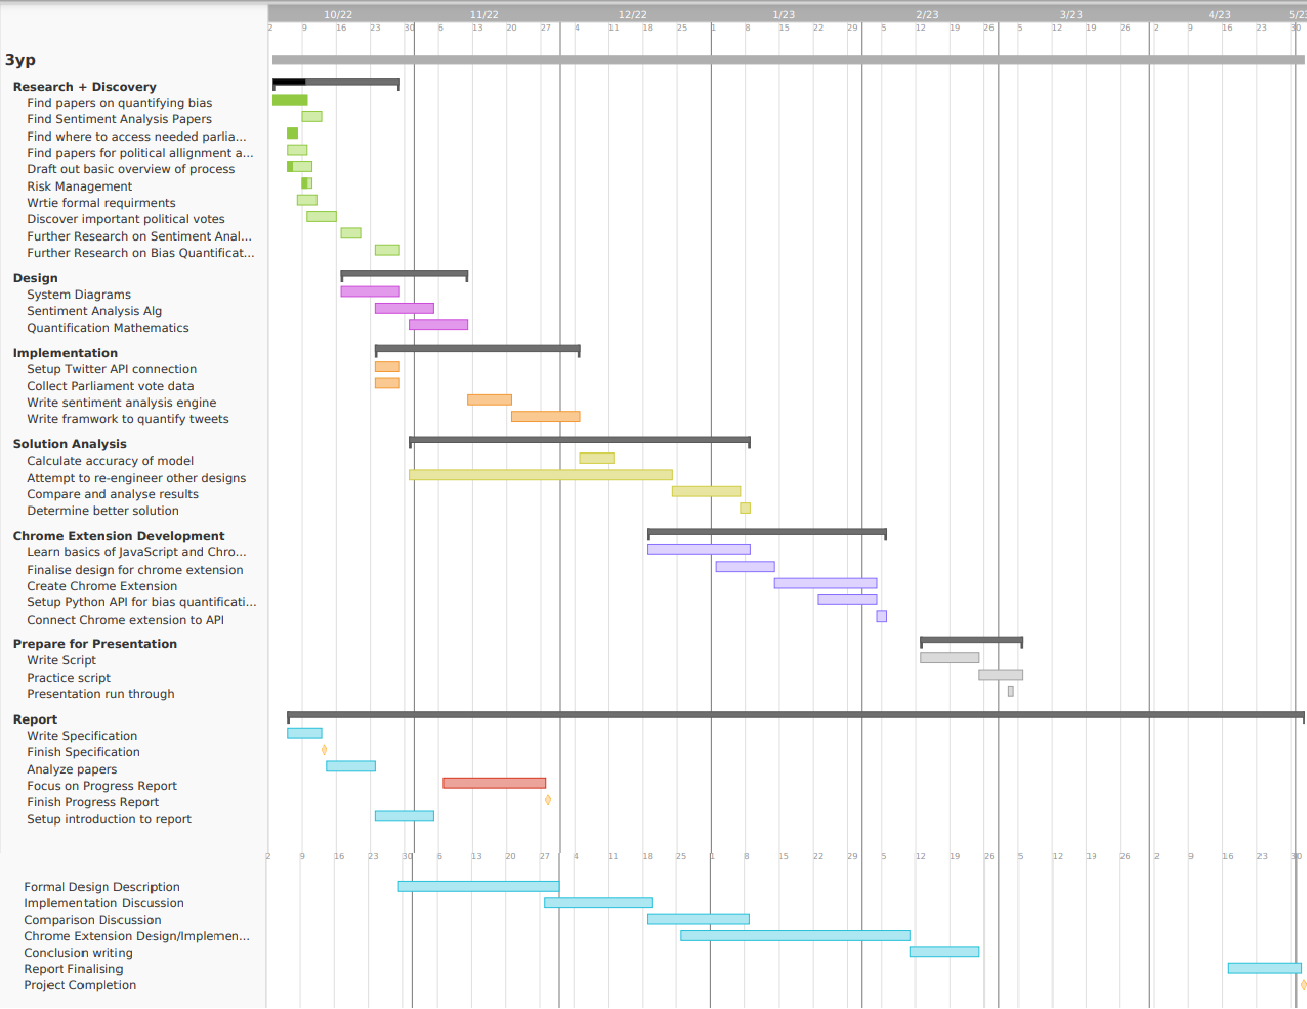
\includegraphics[width=150mm]{../images/3yp timeline.png}
    \caption{Project Timeline}
    \label{fig:timeline}
\end{figure}

\section{Risk Management}
\label{sec:risk}
There are several factors that pose a risk to this project. Below is a table to illustrate what risks are prevalent, how big of an impact they will have, and how to counteract these risks.\\
The scores are ranked from 1-5. 5=high, 1=low.\\
\newpage
\begin{table}[htbp]
    \begin{tabular}{|p{25mm}|p{20mm}|p{13mm}|p{55mm}|p{14mm}|}
    \hline
        Risk & Likelihood of Occurring & Impact to Project & Impact Mitigation & New Impact \\
        \hline
        Personal issue causing delay in schedule & 4 & 3 & I have purposefully planned my project with room to & 1 \\
        \hline
        Chosen design philosophy fails to produce useful bias metrics & 3 & 4 & Firstly, this project is mainly research based, so no matter the outcome we will gain something from the comparison between approaches. For the Software side of the project we could instead use an already known method if ours does not work. & 2 \\
        \hline
        Changes to Twitter API & 2 & 1 & Any changes to the API should not dramatically affect this project. At worse it could involve some minor code refactoring to correct endpoints/REST queries. & 1\\
        \hline
        Laptop dies & 1 & 5 & Using git+github for version control throughout this project (for code and report), no matter what happens to my own laptop, the codebase will be accessible from any machine & 1\\
        \hline
        Unable to recreate other papers methods & 4 & 4 & Instead, I can take the papers results as true (after analysis of results credibility). I can also just create the chrome extension using my own method & 1\\
        \hline
    \end{tabular}
    \caption{Possible risks}
    \label{tab:risk}
\end{table}

\newpage
\bibliographystyle{../common/plainnat}
\bibliography{../common/bibliography}

\end{document}
